\documentclass[tikz]{standalone}
\usepackage{tikz}
\usetikzlibrary{shapes, arrows, positioning}

\begin{document}

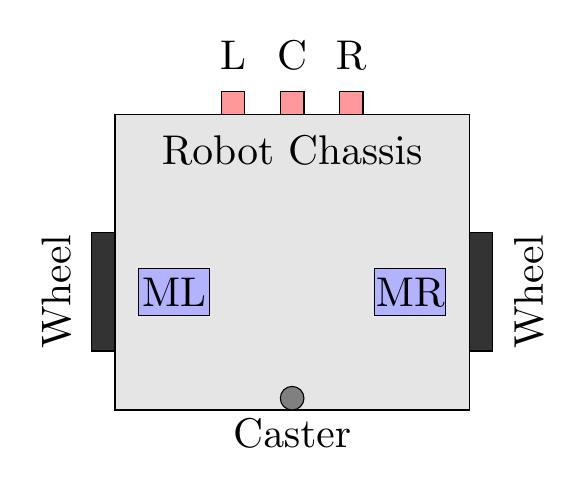
\begin{tikzpicture}[scale=1.5, every node/.style={transform shape}]
    % Chassis
    \draw[fill=gray!20] (-1.5,-1) rectangle (1.5,1.5);
    \node at (0,1.2) {Robot Chassis};

    % Wheels
    \draw[fill=black!80] (-1.7,-0.5) rectangle (-1.5,0.5);
    \draw[fill=black!80] (1.5,-0.5) rectangle (1.7,0.5);
    \node[rotate=90] at (-2,0) {Wheel};
    \node[rotate=90] at (2,0) {Wheel};


    % Motors
    \draw[fill=blue!30] (-1.3, -0.2) rectangle (-0.7, 0.2);
    \draw[fill=blue!30] (0.7, -0.2) rectangle (1.3, 0.2);
    \node at (-1,0) {ML};
    \node at (1,0) {MR};

    % Sensors
    \draw[fill=red!40] (-0.6, 1.5) rectangle (-0.4, 1.7);
    \draw[fill=red!40] (-0.1, 1.5) rectangle (0.1, 1.7);
    \draw[fill=red!40] (0.4, 1.5) rectangle (0.6, 1.7);
    \node at (-0.5,2) {L};
    \node at (0,2) {C};
    \node at (0.5,2) {R};
    
    % Caster Wheel
    \draw[fill=black!50] (0, -0.9) circle (0.1);
    \node at (0,-1.2) {Caster};

\end{tikzpicture}


\end{document}
